\section{仿射簇之间的多项式映射}\label{sec:polynomial-maps-between-affine-varieties}

上一章介绍了仿射簇 $X\subseteq\mathbb{A}^{m}$ 的坐标环 $K[X]$, 其元素是多项式函数 $F:X\to K$. 把 $K$ 与 $\mathbb{A}^{1}$ 等同, 就可以把这类函数看成仿射簇之间的映射的特例 (即 $X$ 到 $\mathbb{A}^{1}$ 的映射). 我们的第一个目标是扩充这一定义, 使它涵盖从任意仿射簇到另一个仿射簇的映射.

\BookPairedNoteLeft
  {这里有意区分\textquotedbl{}函数\textquotedbl{}和\textquotedbl{}映射\textquotedbl{}两个词. 函数在基域中取值, 而映射在仿射簇中取值.}
  {设 $X\subseteq\mathbb{A}^{m}$ 是仿射簇. 因为坐标环 $K[X]$ 的每个元素都是函数 $X\to K$, 所以 $n$ 个元素 $F_{1},\ldots,F_{n}\in K[X]$ 给出一个映射 $X\to\mathbb{A}^{n}$, 定义为 $a\in X\mapsto(F_{1}(a),\ldots,F_{n}(a))\in\mathbb{A}^{n}$.}
\noindent 若 $Y\subseteq\mathbb{A}^{n}$ 为仿射簇, 且映射 $X\to\mathbb{A}^{n}$ 的像恰好落在 $Y$ 中, 就得到映射 $X\to Y$. 这样由多项式函数给出的映射称为多项式映射.

\begin{Definition}{仿射簇之间的多项式映射}\leavevmode\label{def:polynomial-map-between-affine-varieties}
  设 $X\subseteq\mathbb{A}^{m}$ 与 $Y\subseteq\mathbb{A}^{n}$ 为仿射簇. 若存在 $F_{1},\ldots,F_{n}\in K[X]$, 使得对每个 $a\in X$ 都有
  \[
    F(a)=(F_{1}(a),\ldots,F_{n}(a)),
  \]
  则称映射 $F:X\to Y$ 是\textbf{多项式映射}.
\end{Definition}

特别地, $X$ 上的多项式函数与多项式映射 $F:X\to\mathbb{A}^{1}$ 是完全相同的概念. 在下一例中, 我们考虑一个陪域是仿射空间 $\mathbb{A}^{3}$ 的多项式映射.

\begin{Example}{到仿射空间的多项式映射}\leavevmode\label{ex:polynomial-map-to-affine-space}
  考虑抛物线 $X=\mathcal{V}(x_{2}-x_{1}^{2})\subseteq\mathbb{A}^{2}$. (为给下一例作准备, 这里将变量记为 $x_{1},x_{2}$, 而不是 $x,y$.) 那么
  \[
    \begin{aligned}
      F:X&\to\mathbb{A}^{3}\\
      (a_{1},a_{2})&\mapsto(a_{1}-a_{1}^{2},a_{1}+a_{2},a_{1}^{2}-a_{2}^{2})
    \end{aligned}
  \]
  是多项式映射, 因为它的三个分量函数
  \[
    F_{1}(a_{1},a_{2})=a_{1}-a_{1}^{2},\quad F_{2}(a_{1},a_{2})=a_{1}+a_{2},
    \quad\text{以及}\quad F_{3}(a_{1},a_{2})=a_{1}^{2}-a_{2}^{2}
  \]
  分别来自多项式
  \[
    f_{1}=x_{1}-x_{1}^{2},\quad f_{2}=x_{1}+x_{2},\quad\text{以及}\quad f_{3}=x_{1}^{2}-x_{2}^{2},
  \]
  因而都是 $K[X]$ 的元素. 注意, 三个多项式
  \[
    g_{1}=x_{1}-x_{2},\quad g_{2}=x_{1}+x_{1}^{2},\quad\text{以及}\quad g_{3}=x_{2}-x_{2}^{2}
  \]
  给出同一个多项式映射 $F:X\to\mathbb{A}^{3}$, 因为 $[f_{i}]=[g_{i}]\in K[X]$.
\end{Example}

若 $X\subseteq\mathbb{A}^{m}$ 是仿射簇, 构造陪域为仿射空间的多项式映射 $F:X\to\mathbb{A}^{n}$ 并不困难. 具体来说, 任取多项式 $f_{1},\ldots,f_{n}\in K[x_{1},\ldots,x_{m}]$, 令
\[
  F_{i}=[f_{i}]\in\frac{K[x_{1},\ldots,x_{m}]}{\mathcal{I}(X)}=K[X],
\]
就定义了这种映射的坐标函数 $F_{1},\ldots,F_{n}$. 另一组选取的多项式 $g_{1},\ldots,g_{n}$ 给出同一个多项式映射, 当且仅当对每个 $i$ 都有 $f_{i}-g_{i}\in\mathcal{I}(X)$.

另一方面, 若 $Y\subsetneq\mathbb{A}^{n}$ 是不同于整个仿射空间的仿射簇, 那么并非每一组 $F_{1},\ldots,F_{n}\in K[X]$ 都给出映射 $F:X\to Y$. 特别地, 要保证 $X$ 中每个点的像都是 $Y$ 中的点, 必须要求对每个 $a\in X$, 点
\[
  (F_{1}(a),\ldots,F_{n}(a))\in\mathbb{A}^{n}
\]
确实落在 $Y$ 中, 即为 $Y$ 的定义多项式的零点. 更具体地, 若 $Y=\mathcal{V}(S)$, 其中 $S\subseteq K[x_{1},\ldots,x_{n}]$, 那么必须验证对每个 $a\in X$ 与每个 $g\in S$, 都有
\[
  g(F_{1}(a),\ldots,F_{n}(a))=0.
\]

\begin{Example}{到仿射簇的一个多项式映射}\leavevmode\label{ex:parabola-map-to-hyperbolic-paraboloid}
  \BookPairedFigure
    {和 Example~\ref{ex:polynomial-map-to-affine-space} 一样, 设 $X=\mathcal{V}(x_{2}-x_{1}^{2})\subseteq\mathbb{A}^{2}$, 但现在令 $Y=\mathcal{V}(y_{1}y_{2}-y_{3})\subseteq\mathbb{A}^{3}$. 在实数上, $Y$ 是\hyperref[fig:curve-on-hyperbolic-paraboloid]{右图}所示的双曲抛物面, 而 Example~\ref{ex:polynomial-map-to-affine-space} 中的函数
    \[
      \begin{aligned}
        F:X&\to Y\\
        (a_{1},a_{2})&\mapsto(a_{1}-a_{1}^{2},a_{1}+a_{2},a_{1}^{2}-a_{2}^{2})
      \end{aligned}
    \]
    是从 $X$ 到 $Y$ 的多项式映射, 它的像就是图中曲面上的那条曲线.}
    {\phantomsection\label{fig:curve-on-hyperbolic-paraboloid}%
      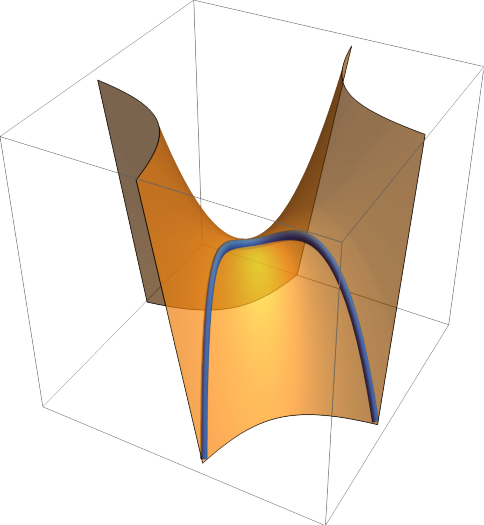
\includegraphics[width=\linewidth]{figures/curve-on-hyperbolic-paraboloid.png}}
  \noindent 我们已经验证 $F$ 的三个分量函数都是多项式函数, 但现在还必须确认其像确实落在 $Y$ 中. 这等价于断言 $F(a_{1},a_{2})$ 满足 $Y$ 的定义方程 $y_{1}y_{2}-y_{3}$, 换句话说, 只要 $(a_{1},a_{2})\in X$, 就有
  \[
    F_{1}(a_{1},a_{2})F_{2}(a_{1},a_{2})-F_{3}(a_{1},a_{2})=0.
  \]
  为验证这一点, 只需代入 $F_{1},F_{2},F_{3}$ 的表达式并整理:
  \[
    (a_{1}-a_{1}^{2})(a_{1}+a_{2})-(a_{1}^{2}-a_{2}^{2})
       =(a_{1}+a_{2})(a_{2}-a_{1}^{2})=(a_{1}+a_{2})\cdot0=0,
  \]
  其中第二个等号来自 $(a_{1},a_{2})\in X$, 它蕴含 $a_{2}-a_{1}^{2}=0$.
\end{Example}

\BookPairedNoteLeft
  {为区分 $X$ 与 $Y$ 上的坐标, 常像上一例那样使用下标: 对 $X$ 用 $x_{1},x_{2},\ldots$, 对 $Y$ 用 $y_{1},y_{2},\ldots$.}
  {读者从代数中已经熟悉这样的概念: 某些同态是同构, 而同构的对象具有一切有关的共同性质. 例如, 同构的群具有相同的群论性质.}
\noindent 类似地, 仿射簇的同构使我们能够讨论仿射簇在本质上相同是什么意思.

\begin{Definition}{仿射簇的同构}\leavevmode\label{def:isomorphism-of-affine-varieties}
  设 $X\subseteq\mathbb{A}^{m}$ 与 $Y\subseteq\mathbb{A}^{n}$ 为仿射簇. 若多项式映射 $F:X\to Y$ 有一个同样为多项式映射的逆函数 $F^{-1}:Y\to X$, 则称 $F$ 是一个\textbf{同构}. 若存在这样的同构, 则称 $X$ 与 $Y$ \textbf{同构}, 记作 $X\cong Y$.
\end{Definition}

\begin{Example}{抛物线同构于 $\mathbb{A}^{1}$}\leavevmode\label{ex:parabola-isomorphic-to-affine-line}
  \BookPairedFigure
    {设 $X=\mathcal{V}(x_{2}-x_{1}^{2})\subseteq\mathbb{A}^{2}$. 注意, 由下式定义的两个映射 $F$ 与 $G$
    \[
      \begin{aligned}
        F:X&\to\mathbb{A}^{1}&G:\mathbb{A}^{1}&\to X\\
        (a_{1},a_{2})&\mapsto a_{1}&b&\mapsto(b,b^{2})
      \end{aligned}
    \]
    都是多项式映射.}
    {\phantomsection\label{fig:parabola-isomorphism}%
      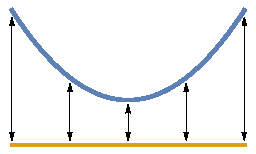
\includegraphics[width=\linewidth]{figures/parabola-isomorphism.pdf}}
  \noindent 此外, 容易验证 $F\circ G$ 是 $\mathbb{A}^{1}$ 上的恒等映射. 利用对每个 $(a_{1},a_{2})\in X$ 都有 $a_{2}=a_{1}^{2}$, 也可以验证 $G\circ F$ 是 $X$ 上的恒等映射. 因而 $X\cong\mathbb{A}^{1}$. \hyperref[fig:parabola-isomorphism]{上图}画出了 $\mathbb{R}$ 上仿射直线与抛物线之间的同构, 其中 $F$ 是向下的映射, $G$ 是向上的映射.
\end{Example}

\begin{Example}{给出同构的投影}\leavevmode\label{ex:isomorphic-projections}
  推广上一例, 假设 $X=\mathcal{V}(x_{m}-g)\subseteq\mathbb{A}^{m}$, 其中 $g\in K[x_{1},\ldots,x_{m-1}]$. 考虑两个映射
  \[
    \begin{aligned}
      F:X&\to\mathbb{A}^{m-1}\\
      (a_{1},\ldots,a_{m})&\mapsto(a_{1},\ldots,a_{m-1})
    \end{aligned}
  \]
  以及
  \[
    \begin{aligned}
      G:\mathbb{A}^{m-1}&\to X\\
      (b_{1},\ldots,b_{m-1})&\mapsto(b_{1},\ldots,b_{m-1},g(b_{1},\ldots,b_{m-1})).
    \end{aligned}
  \]
  $F$ 与 $G$ 都是多项式映射. 利用对每个 $(a_{1},\ldots,a_{m})\in X$ 都有 $a_{m}=g(a_{1},\ldots,a_{m-1})$, 可见两者互为逆映射. 因而 $X\cong\mathbb{A}^{m-1}$. 本例的进一步推广见 Exercise~\ref{ex:eliminate-a-linear-coordinate}.
\end{Example}

\begin{Example}{平移是同构}\leavevmode\label{ex:translation-is-iso}
  给定参考点 $c=(c_{1},\ldots,c_{m})\in\mathbb{A}^{m}$, 考虑平移映射
  \[
    \begin{aligned}
      T_{c}:\mathbb{A}^{m}&\to\mathbb{A}^{m}\\
      (a_{1},\ldots,a_{m})&\mapsto(a_{1}+c_{1},\ldots,a_{m}+c_{m}).
    \end{aligned}
  \]
  那么对任意仿射簇 $X\subseteq\mathbb{A}^{m}$, 平移 $T_{c}(X)$ 也是仿射簇. 为见此点, 注意多项式 $f(x_{1},\ldots,x_{m})$ 在 $T_{c}(X)$ 上处处为零, 当且仅当 $f(x_{1}+c_{1},\ldots,x_{m}+c_{m})$ 在 $X$ 上处处为零, 所以
  \[
    T_{c}(X)=\mathcal{V}\bigl(\{f\in K[x_{1},\ldots,x_{n}]
      \mid f(x_{1}+c_{1},\ldots,x_{m}+c_{m})\in\mathcal{I}(X)\}\bigr).
  \]
  映射 $T_{c}:X\to T_{c}(X)$ 显然是多项式映射, 而且实际上还是同构. 为证明这一点, 只需注意它有一个多项式逆映射, 即用参考点 $(-c_{1},\ldots,-c_{m})\in\mathbb{A}^{m}$ 作反向平移.

  Exercise~\ref{ex:invertible-affine-linear-map} 把本例推广到平移和可逆线性映射的复合; 这样的复合称为\textbf{仿射线性变换}.
\end{Example}

\BookPairedNote
  {仿射簇的映射要成为同构, 就必须是双射, 因为这是逆函数存在的必要条件. 然而, \emph{并非每个双射的仿射簇多项式映射都是同构}, 因为逆函数即使存在也未必是多项式映射.}
  {几何和代数在这里有所不同: 在代数中, 若同态 (群, 环, 代数等的同态) 有逆函数, 那么这个逆函数自动是同态. 见 Exercise~\ref{ex:bijective-k-algebra-homomorphism-is-isomorphism}.}
\noindent 下一例说明这一现象.

\begin{Example}{双射的多项式映射未必是同构}\leavevmode\label{ex:cusp-bijective-map-not-isomorphism}
  \BookPairedFigure
    {考虑 $X=\mathcal{V}(x^{2}-y^{3})\subseteq\mathbb{A}^{2}$. 那么
    \[
      \begin{aligned}
        F:\mathbb{A}^{1}&\to X\\
        a&\mapsto(a^{3},a^{2})
      \end{aligned}
    \]
    是\hyperref[fig:cusp-polynomial-map]{右图}所示的多项式映射. (注意, 对每个 $a\in\mathbb{A}^{1}$, 点 $(a^{3},a^{2})\in\mathbb{A}^{2}$ 确实满足方程 $x^{2}-y^{3}=0$.)}
    {\phantomsection\label{fig:cusp-polynomial-map}%
      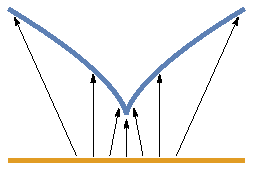
\includegraphics[width=\linewidth]{figures/cusp-polynomial-map.pdf}}
  \noindent 此外, 读者可以验证 $F$ 的一个逆函数为
  \[
    \begin{aligned}
      G:X&\to\mathbb{A}^{1}\\
      (b,c)&\mapsto
       \begin{cases}
         b/c & \text{若 }c\ne0,\\
         0   & \text{若 }c=0.
       \end{cases}
    \end{aligned}
  \]
  然而, $G$ 不是多项式映射. $G$ 涉及对输入作除法, 这的确暗示它可能不是多项式映射. 但如 Example~\ref{ex:apparently-nonpolynomial-hyperbola-function} 所示, 要确定 $G$ 不是多项式映射, 仍需更加谨慎. 下一节将建立证明 $X\not\cong\mathbb{A}^{1}$ 所需的工具, 由此可知 $G$ 不可能是多项式映射. 曲线 $X$ 似乎改变方向的\textquotedbl{}尖点\textquotedbl{}给出了 $X\not\cong\mathbb{A}^{1}$ 的一个直观线索.
\end{Example}

要证明 $X\cong Y$, 做法相对直接: 必须找到 $X$ 与 $Y$ 之间的一个同构. 但证明 $X\not\cong Y$ 更微妙. 怎样严格证明不存在任何同构? 在代数中, 我们有不少工具做这件事: 要证明两个环不同构, 可以找到某种一个环具有而另一个不具有的环论性质, 例如是整环或者是 UFD.

因此, 如果想要判定何时两个仿射簇不同构, 一个自然的办法是证明 $X\cong Y$ 蕴含 $K[X]\cong K[Y]$. 一旦做到这一点, 证明 $K[X]\not\cong K[Y]$ 的代数论证就会蕴含几何结论 $X\not\cong Y$, 于是可以用代数方法判定何时仿射簇不同构. 因而, 我们的目标是建立一个过程, 将仿射簇的同构转换成对应坐标环的同构. 这个过程就是拉回, 是下一节的主题.

\BookExerciseHeading
\begin{BookExercises}
  \item\label{ex:polynomial-map-to-two-equation-variety} 设 $X=\mathcal{V}(y^{2}-z^{2}+xy-z,z^{2}-x^{3}y^{2})\subseteq\mathbb{A}^{3}$. 证明 $F(a)=(1,a,a)$ 定义了多项式映射 $F:\mathbb{A}^{1}\to X$. $F$ 是同构吗?
  \item\label{ex:polynomial-map-between-two-circles} 设 $X=\mathcal{V}(x^{2}+y^{2}-1)\subseteq\mathbb{A}^{2}$, 并设 $Y=\mathcal{V}(u^{2}+v^{2}-2)\subseteq\mathbb{A}^{2}$. 证明 $F(a,b)=(a+b,a-b)$ 定义了多项式映射 $F:X\to Y$. $F$ 是同构吗?
  \item\label{ex:polynomial-map-to-nodal-cubic} 设 $X=\mathcal{V}(y^{2}-x^{3}-x^{2})\subseteq\mathbb{A}^{2}$. 证明 $F(a)=(a^{2}-1,a^{3}-a)$ 定义了多项式映射 $F:\mathbb{A}^{1}\to X$. $F$ 是同构吗? (提示: 画图.)
  \item\label{ex:eliminate-a-linear-coordinate} 设 $X=\mathcal{V}(f_{1},\ldots,f_{k},x_{m}-g)\subseteq\mathbb{A}^{m}$, 其中 $g\in K[x_{1},\ldots,x_{m-1}]$, $f_{1},\ldots,f_{k}\in K[x_{1},\ldots,x_{m}]$. 对每个 $i=1,\ldots,k$, 定义
    \[
      \widetilde{f}_{i}=f_{i}(x_{1},\ldots,x_{m-1},g)\in K[x_{1},\ldots,x_{m-1}],
    \]
    并令 $Y=\mathcal{V}(\widetilde{f}_{1},\ldots,\widetilde{f}_{k})\subseteq\mathbb{A}^{m-1}$. 证明 $X\cong Y$. (这说明如果一个仿射簇的某个定义方程对其中一个变量是线性的, 那么就可以用一个与之同构的仿射簇取代它, 新簇由更少变量中的更少方程定义.)
  \item\label{ex:polynomial-image-may-not-be-variety}
    \begin{enumerate}[label=(\alph*)]
      \item 证明多项式映射
        \[
          \begin{aligned}
            F:\mathbb{A}^{1}&\to\mathbb{A}^{3}\\
            a&\mapsto(a,a^{2},a^{3})
          \end{aligned}
        \]
        的像是仿射簇.
      \item 证明多项式映射
        \[
          \begin{aligned}
            G:\mathbb{A}^{2}&\to\mathbb{A}^{2}\\
            (a,b)&\mapsto(a,ab)
          \end{aligned}
        \]
        的像不是仿射簇.
    \end{enumerate}
    因此, 多项式映射的像可能是仿射簇, 也可能不是.
  \item\label{ex:invertible-affine-linear-map} 设 $M$ 是一个系数在 $K$ 中的可逆 $m\times m$ 矩阵, 且 $c\in\mathbb{A}^{m}$. 将 $\mathbb{A}^{m}$ 与向量空间 $K^{m}$ 等同, 并将 $M$ 与线性变换 $\phi_{M}:K^{m}\to K^{m}$ 等同, 定义函数
    \[
      \begin{aligned}
        F:\mathbb{A}^{m}&\to\mathbb{A}^{m}\\
        a&\mapsto\phi_{M}(a)+c.
      \end{aligned}
    \]
    证明下列结论.
    \begin{enumerate}[label=(\alph*)]
      \item 若 $X\subseteq\mathbb{A}^{m}$ 是仿射簇, 则 $F(X)\subseteq\mathbb{A}^{m}$ 是仿射簇.
      \item 若 $X\subseteq\mathbb{A}^{m}$ 是仿射簇, 则 $X\cong F(X)$.
    \end{enumerate}
  \item\label{ex:linear-equations-give-affine-space} 设 $X=\mathcal{V}(\ell_{1},\ldots,\ell_{k})\subseteq\mathbb{A}^{n}$, 其中每个 $\ell_{i}$ 都是线性多项式:
    \[
      \ell_{i}=a_{i1}x_{1}+\cdots+a_{in}x_{n}+b_{i}\in K[x_{1},\ldots,x_{n}].
    \]
    令 $M=(a_{ij})$ 为 $k\times n$ 的系数矩阵. 假设 $X$ 非空, 证明
    \[
      X\cong\mathbb{A}^{n-\operatorname{rk}(M)}.
    \]
    (提示: 使用秩--零度定理.)
\end{BookExercises}

\par\smallskip
{\footnotesize
\noindent\textbf{开放获取.} 本章按照
\href{http://creativecommons.org/licenses/by-nc/4.0/}{Creative Commons Attribution-NonCommercial 4.0 International License}
的条款授权. 该许可允许以任何媒介或格式进行非商业性使用, 分享, 改编, 分发和复制, 但须对原作者和来源作适当署名, 提供 Creative Commons 许可的链接, 并说明是否作了修改.

\noindent
\begin{minipage}[t]{.17\linewidth}
  \vspace{0pt}
\includegraphics[width=.9\linewidth]{figures/source-cc-by-nc.png}
\end{minipage}\hfill
\begin{minipage}[t]{.81\linewidth}
  \vspace{0pt}本章的图片或其他第三方材料均纳入本章的 Creative Commons 许可, 除非材料的署名行另有注明. 如果材料未纳入本章的 Creative Commons 许可, 且您拟进行的使用未获法律规定的许可或超出允许使用的范围, 则须直接向著作权持有人取得许可.
\end{minipage}\par}
